\documentclass{article}
\usepackage{indentfirst}
\usepackage{ctex}
\usepackage{geometry}
\usepackage{enumerate}
\usepackage{amssymb, amsmath}
\usepackage{algorithm,algorithmic}
\usepackage{listings}
\usepackage{graphicx, subfigure}
\usepackage{caption2}
\usepackage{booktabs}
\usepackage{dirtree}
\usepackage{fontspec}
\usepackage{color}
\usepackage{hyperref}

%\geometry{left=3.17cm,right=3.17cm,top=2.54cm,bottom=2.54cm} % 页边距
\geometry{left=2.54cm,right=2.54cm,top=2.17cm,bottom=2.17cm} % 页边距

\definecolor{Gainsboro}{RGB}{220,220,220}
\definecolor{SlateBlue}{RGB}{106,90,205}

\hypersetup{hidelinks} % 超链接不显示方框

\lstset{ % 设置 lstlisting 代码风格
	language=Go,
	basicstyle=\sffamily\tiny,
	%numbers=left,
	flexiblecolumns,
	%frame=lrtb, % 边框
	backgroundcolor=\color{Gainsboro},
}

\newcommand{\code}[1]{{~\fontspec{Book Antiqua}\textcolor{SlateBlue}{#1}~}}% ~是空格

\begin{document}
	
\title{LevelDB、InfluxDB性能对比}
\date{}
\maketitle

\section{测试环境}
\begin{small}
\begin{itemize}
	\item OS:Ubuntu 18.04.5 LTS x86\_64 GNU/Linux
	\item CPU:Intel(R) Xeon(R) CPU E5-2678 v3 @ 2.50GHz
	\item Memory:64G
	\item Disk:Samsung SSD 860 EVO 500GB
\end{itemize}
\end{small}

\section{测试及结论}
\subsection{初步测试}
\subsubsection{InfluxDB}
data points结构:
\begin{small}
\begin{itemize}
	\item measurement: ``temp''
	\item tag set: ``machine''和``type''均为30字节的字符串
	\item field set: ``external''和``internal''均为4096字节的字符串
\end{itemize}
\end{small}

按照influxdb的kv数据模型,上述一个data point可分解为两条kv数据,KeySize = 91B,ValueSize = 4104B,一条kv数据的总大小为4195B。

测试程序使用的是异步API进行写入,batch size = 100,也就是每100个points为一个写入批次,相当于200条kv数据。测试程序持续地写入50万个points,相当于100万条kv数据,influxdb的平均吞吐量为\textbf{2008 points/s},即$2008*2*4195/2^{20}$=\textbf{16.1 MB/s}。

上述测试结果是在未开启TSI索引的情况,经测试,TSI开启与否并不会对吞吐量造成明显影响,原因是TSI的尺寸较小。

\subsubsection{LevelDB}
为了让 leveldb 的测试数据规模和 influxdb 相当,需要修改测试程序 db\_bench 的参数设置。

首先是 kv 数据的大小,db\_bench 使用的 KeySize = 16 B,ValueSize = 100 B,由于 leveldb 固定了 key 的大小,所以只能将 value 的大小修改为 4195-16=4179B,使得 kv 数据的总大小和 influxdb 相当。

其次是写入模式,``fillbatch''模式和 influxdb 测试程序的异步写最为相似,默认 batch size = 1000,需将其修改为 200 (与 influxdb 测试程序相当,注意这里的 batch size 是以 kv 数据为准)。

测试程序以"fillbatch"模式持续地写入 100 万条 kv 数据的结果如下:
\begin{lstlisting}
# ./db_bench --num=1000000 --benchmarks="fillbatch" --db="benchdb" --use_existing_db=0
LevelDB:    version 1.22
Date:       Wed Apr 14 20:16:02 2021
CPU:        48 * Intel(R) Xeon(R) CPU E5-2678 v3 @ 2.50GHz
CPUCache:   30720 KB
Keys:       16 bytes each
Values:     4179 bytes each (2090 bytes after compression)
Entries:    1000000
RawSize:    4000.7 MB (estimated)
FileSize:   2008.0 MB (estimated)
------------------------------------------------
fillbatch    :      78.995 micros/op;   50.6 MB/s
\end{lstlisting}

平均吞吐量是\textbf{50.6 MB/s}

根据对 db\_bench 源代码的分析可知,这里显示的吞吐量是原始 kv 数据的吞吐量,和 influxdb 测试程序给出的结果含义一致。

\subsubsection{初步结论}
在不考虑网络 IO 延迟的情况下,leveldb 的写入性能为 influxdb 的3倍多。至于这个结论是否准确、测试程序给出的吞吐量是否是各自存储引擎的极限,则需要进一步测试。

\subsection{进一步测试}
进一步测试的目的是要测出 influxdb 和 leveldb 的极限吞吐量,只有这样才能反映出各自真实的性能。

\subsubsection{InfluxDB}
初步测试中只启动了一个 influxdb 客户端进程进行写入,所以客户端是单线程写。下面分别启动2个和4个客户端进程向服务端发起写请求,均摊地写入 50 万个 points(相当于 100 万条 kv 数据)。

\subsubsection*{2个线程}
把两个测试程序的给出吞吐量加起来可得总吞吐量为 1712+1724=\textbf{3436 points/s}=\textbf{27.5 MB/s}

\subsubsection*{4个线程}
932+932+939+939=\textbf{3742 points/s}=\textbf{29.9 MB/s}

\subsubsection*{综上,可以认为客户端使用4个写线程时 influxdb 的吞吐量达到极限:29.9 MB/s}

\subsubsection{LevelDB}
db\_bench 程序的源代码中变量\code{FLAGS\_threads}表示写线程的数量,默认为1;将其分别修改为2和4后再词测试,结果如下:

\subsubsection*{2个线程}
\begin{lstlisting}
# ./db_bench --num=1000000 --benchmarks="fillbatch" --db="benchdb"
LevelDB:    version 1.22
Date:       Wed Apr 14 20:59:06 2021
CPU:        48 * Intel(R) Xeon(R) CPU E5-2678 v3 @ 2.50GHz
CPUCache:   30720 KB
Keys:       16 bytes each
Values:     4179 bytes each (2090 bytes after compression)
Entries:    1000000
RawSize:    4000.7 MB (estimated)
FileSize:   2008.0 MB (estimated)
------------------------------------------------
fillbatch    :      97.062 micros/op;   82.4 MB/s
\end{lstlisting}
平均吞吐量为\textbf{82.4 MB/s},和单线程相比有明显提升

\subsubsection*{4个线程}
\begin{lstlisting}
➜  build git:(master) ✗ ./db_bench --num=1000000 --benchmarks="fillbatch" --db="benchdb"
LevelDB:    version 1.22
Date:       Wed Apr 14 21:03:30 2021
CPU:        48 * Intel(R) Xeon(R) CPU E5-2678 v3 @ 2.50GHz
CPUCache:   30720 KB
Keys:       16 bytes each
Values:     4179 bytes each (2090 bytes after compression)
Entries:    1000000
RawSize:    4000.7 MB (estimated)
FileSize:   2008.0 MB (estimated)
------------------------------------------------
fillbatch    :     334.212 micros/op;   47.9 MB/s
\end{lstlisting}
平均吞吐量为\textbf{47.9 MB/s},不及单线程的性能

\subsubsection*{综上,可以认为 leveldb 的极限吞吐量为82.4 MB/s}

\subsection{性能对比}
下表是 influxdb 和 leveldb 在相同写负载(100 万条相同大小的 kv 数据)下的性能对比:

\begin{table}[htbp]
	\centering
	\begin{tabular}{rrrr}
		\toprule
		写线程数 & 1 & 2 & 4 \\
		\midrule
		InfluxDB & 16.1 MB/s & 27.5 MB/s & \textbf{29.9 MB/s} \\
		LevelDB & 50.6 MB/s & \textbf{82.4 MB/s} & 47.9 MB/s \\
		\bottomrule
	\end{tabular}
\end{table}

\section{测试结果分析}
在相同写负载下,leveldb 的最大吞吐量(82.4 MB/s)是 influxdb 最大吞吐量(29.9 MB/s)的 3 倍多。对于如此大的差异,我们从二者的源码中找到了答案,即 WAL 日志的刷盘,在 leveldb 测试程序 db\_bench 的``fillbatch''模式下,leveldb 的处理方式是:

对每个批次的写请求,将日志项写到内存缓冲区,当缓冲区满了就调用\code{write}将缓冲区的数据写入文件。但是我们都知道\code{write}只会将数据写到文件数据块在内存中的缓冲页面,并不会直接落盘。有必要梳理一下 Linux 的文件 IO 流程:

\subsubsection*{read}
找到\code{inode}结构(\code{file}结构 ->\code{dentry}结构 -> \code{inode}结构)(\code{file}结构表示文件读写的上下文,例如当前读写位置、访问模式、引用计数等;\code{dentry}结构,目录项,描述文件在 VFS 目录树中的信息;\code{inode}结构是文件在 VFS 中的索引节点),\code{inode}结构记录了文件内容在内存中所对应的缓冲页面。如果缓冲页面不再内存中,就从设备上读入;否则直接读取缓冲页面。这里涉及 Linux 的文件预读技术:当发生顺序读取时,系统会以页面为单位读取比应用程序所要求的更多的数据,将其缓存到\code{inode}结构所记录的缓冲页面中。缓冲页面的管理使用 LRU 替换策略。

\subsubsection*{write}
如前所述,如果欲访问的文件内容已经在缓冲页面中,写操作只是把数据写到缓冲页面中,当 CPU 较空闲时会调度一个内核线程\code{kflushd}完成刷盘。另外,应用程序还可以调用\code{fsync}强制调度内核线程\code{kflushd}将缓冲页面落盘。

\begin{figure}[htbp]
	\centering
	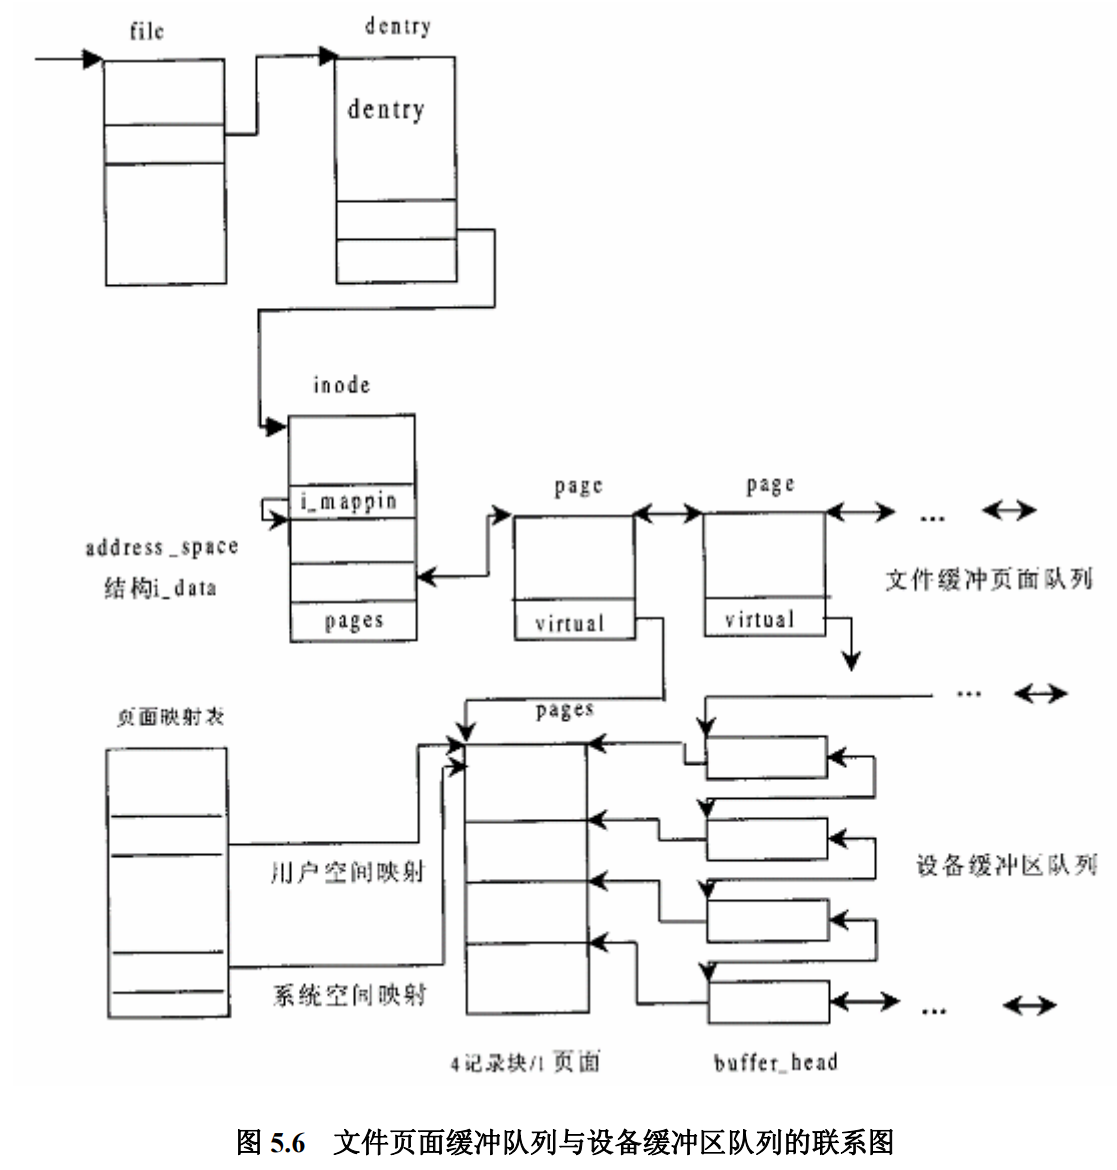
\includegraphics[width=0.6\linewidth]{imgs/文件页面缓冲队列.png}
\end{figure}

leveldb 对于写 WAL 时是否需要将数据落盘的选择权交给了用户,即用户可以指定每写一条 WAL 日志项就将数据 fsync 到磁盘上。不幸的是,在 db\_bench 除了``fillsync''的其他写入模式下,这个 sync 选项没有被打开。但是 influxdb 写 WAL 日志的动作是,每当有日志项写入后,都要将数据 fsync 到磁盘上,而且是强制性的,没有给用户留有选择的余地。

在 db\_bench 的``fillbatch''模式里把 WAL 的 sync 选项打开,把前面的测试重做一遍,得到如下结果:

\begin{table}[htbp]
	\centering
	\begin{tabular}{rrrr}
			\toprule
		写线程数 & 1 & 2 & 4 \\
		\midrule
		InfluxDB & 16.1 MB/s & 27.5 MB/s & \textbf{29.9 MB/s} \\
		LevelDB (WAL sync=false) & 50.6 MB/s & \textbf{82.4 MB/s} & 47.9 MB/s \\
		LevelDB (WAL sync=true) & 32.3 MB/s & \textbf{36.8 MB/s} & 29.9 MB/s \\
		\bottomrule
	\end{tabular}
\end{table}

可以看到,如果打开LevelDB WAL的sync选项,LevelDB的极限吞吐量只比InfluxDB大(36.8-29.9)/29.9=23.1\%

\section{InfluxDB和LevelDB写WAL日志的调度流程}
\subsection{InfluxDB}
\begin{lstlisting}
func (l *WAL) writeToLog(entry WALEntry) (int, error) {
	......
	syncErr := make(chan error)

	segID, err := func() (int, error) {
		l.mu.Lock()
		defer l.mu.Unlock()
		......
		// write and sync
		if err := l.currentSegmentWriter.Write(entry.Type(), compressed); err != nil {
			return -1, fmt.Errorf("error writing WAL entry: %v", err)
		}

		select {
		case l.syncWaiters <- syncErr:
		default:
			return -1, fmt.Errorf("error syncing wal")
		}
		l.scheduleSync()
		......
		return l.currentSegmentID, nil

	}()
	......
	// schedule an fsync and wait for it to complete
	return segID, <-syncErr
}

// scheduleSync will schedule an fsync to the current wal segment and notify any
// waiting gorutines.  If an fsync is already scheduled, subsequent calls will
// not schedule a new fsync and will be handle by the existing scheduled fsync.
func (l *WAL) scheduleSync() {
	// If we're not the first to sync, then another goroutine is fsyncing the wal for us.
	if !atomic.CompareAndSwapUint64(&l.syncCount, 0, 1) {
		return
	}

	// Fsync the wal and notify all pending waiters
	go func() {
		var timerCh <-chan time.Time

		// time.NewTicker requires a > 0 delay, since 0 indicates no delay, use a closed
		// channel which will always be ready to read from.
		if l.syncDelay == 0 {
			// Create a RW chan and close it
			timerChrw := make(chan time.Time)
			close(timerChrw)
			// Convert it to a read-only
			timerCh = timerChrw
		} else {
			t := time.NewTicker(l.syncDelay)
			defer t.Stop()
			timerCh = t.C
		}
		for {
			select {
			case <-timerCh:
				l.mu.Lock()
				if len(l.syncWaiters) == 0 {
					atomic.StoreUint64(&l.syncCount, 0)
					l.mu.Unlock()
					return
				}

				l.sync()
				l.mu.Unlock()
			case <-l.closing:
				atomic.StoreUint64(&l.syncCount, 0)
				return
			}
		}
	}()
}

// sync fsyncs the current wal segments and notifies any waiters.  Callers must ensure
// a write lock on the WAL is obtained before calling sync.
func (l *WAL) sync() {
	err := l.currentSegmentWriter.sync()
	for len(l.syncWaiters) > 0 {
		errC := <-l.syncWaiters
		errC <- err
	}
}
\end{lstlisting}

\code{WAL.syncWaiters}是一个缓冲区长度为1024的channel,相当于一个fsync的请求队列。对于每一个客户端的写请求,InfluxDB在写WAL日志时最后都会来到\code{(*WAL).writeToLog}函数。当\code{(*WAL).wri\\teToLog}获得互斥锁并调用\code{(*WALSegmentWriter).Write}将数据写到内存缓冲区后就会向\code{WAL.syncW\\aiters}写入\code{syncErr},相当于把自己加入到fsync请求队列中,然后\code{(*WAL).scheduleSync}调度一个fsync将日志数据刷盘。\code{(*WAL).scheduleSync}的流程:如果当前已经有一个go routine正在fsync则立即返回,否则新开一个go routine去fsync。当日志数据全部fsync到磁盘后,\code{(*WAL).sync}会通知\code{WAL.syncWaiters}队列里的发起fsync请求的go routine:日志数据已经fsync完毕(具体的实现就是把\code{WAL.syncWaiters}这个channel里的数据全部读出,又因为里面出来的数据也是channel,所以会把\code{err}写进去,从而唤醒\code{(*WAL).writeToLog}在return语句处\code{<-syncErr}的阻塞)。

InfluxDB采取这样的设计是为了防止日志刷盘在高并发下成为性能瓶颈,对不同线程同时产生的日志数据同一调度一个fsync,而非对每个线程写入的数据单独fsync。这种做法叫做\emph{group commit}。group commit的目的是将每个fsync的成本分摊到多个并发事务的多个提交上。如果有10个事务并行尝试提交,那么我们可以通过一个fsync同时将所有事务的WAL日志数据刷盘,而不是为每个事务执行一个fsync。这可以大大减少fsync的调用需要,从而提高每秒提交的吞吐量。

\subsection{LevelDB}
\begin{lstlisting}
Status DBImpl::Write(const WriteOptions& options, WriteBatch* updates) {
  Writer w(&mutex_);
  w.batch = updates;
  w.sync = options.sync;
  w.done = false;

  MutexLock l(&mutex_);
  writers_.push_back(&w);
  while (!w.done && &w != writers_.front()) {
    w.cv.Wait();
  }
  if (w.done) {
    return w.status;
  }

  // 只有排在队首的线程会来到这里, 其他线程在前面等待通知
  // May temporarily unlock and wait.
  Status status = MakeRoomForWrite(updates == nullptr); // 根据DB状态制定写入策略
  uint64_t last_sequence = versions_->LastSequence();
  Writer* last_writer = &w;
  if (status.ok() && updates != nullptr) {  // nullptr batch is for compactions
    WriteBatch* updates = BuildBatchGroup(&last_writer); // 批量组装队列中的部分写线程的batch, 以便批量写入
    WriteBatchInternal::SetSequence(updates, last_sequence + 1);
    last_sequence += WriteBatchInternal::Count(updates);

    // Add to log and apply to memtable.  We can release the lock
    // during this phase since &w is currently responsible for logging
    // and protects against concurrent loggers and concurrent writes
    // into mem_.
    // 因为只有排在队首的线程在写数据, 其他线程都在等待, 不存在竞争, 所以可以unlock
    {
      mutex_.Unlock();
      status = log_->AddRecord(WriteBatchInternal::Contents(updates)); // 先写log
      bool sync_error = false;
      if (status.ok() && options.sync) {
        status = logfile_->Sync();
        if (!status.ok()) {
          sync_error = true;
        }
      }
      if (status.ok()) {
        status = WriteBatchInternal::InsertInto(updates, mem_); // 再写memtable
      }
      mutex_.Lock();
      if (sync_error) {
        // The state of the log file is indeterminate: the log record we
        // just added may or may not show up when the DB is re-opened.
        // So we force the DB into a mode where all future writes fail.
        RecordBackgroundError(status);
      }
    }
    if (updates == tmp_batch_) tmp_batch_->Clear();

    versions_->SetLastSequence(last_sequence); // 更新sequence number
  }

  // 队列中的所有写线程的写操作已完成, 将其全部唤醒. 需要注意的是, while循环的退出条件并不是
  // 队列为空, 而是遍历到last_writer. 由DBImpl::BuildBatchGroup()可知, last_writer并非
  // 队列中的最后一个写线程, 而是最后一个参与写请求批量组装的写线程. 因为这些写线程的batch已
  // 被批量组装为"updates", 所以说他们的写请求已处理完成, 故将done标记为true, 被唤醒后, 回到
  // DBImpl::Write()最开始的那段代码, 就会因为w.done为true而直接return.
  while (true) {
    Writer* ready = writers_.front();
    writers_.pop_front();
    if (ready != &w) {
      ready->status = status;
      ready->done = true;
      ready->cv.Signal();
    }
    if (ready == last_writer) break;
  }

  // Notify new head of write queue
  // 写线程 w 加入队列时可能因为不在队首而进入等待状态, 但是现在 w 之前的写线程都因为
  // 其提交的写请求已处理完成而被唤醒并出队, 那么 w 此时位于队首, 应将其唤醒.
  if (!writers_.empty()) {
    writers_.front()->cv.Signal();
  }

  return status;
}
\end{lstlisting}

和InfluxDB相比,LevelDB不单是对WAL采用group commit,对Memtable也是如此。位于\code{writers\_}队首的线程会调用\code{BuildBatchGroup}组装一批线程的写操作,也就是将多个线程的数据一起写入WAL和Memtable(如果\code{options.sync=true}还会将日志数据落盘)。当队首线程完成批量写之后会通知该批次等待中的线程(这些线程被唤醒后会立即退出\code{DBImpl::Write})。图\ref{fig:leveldb_writebatch}展示了该过程。

\begin{figure}[htbp]
	\centering
	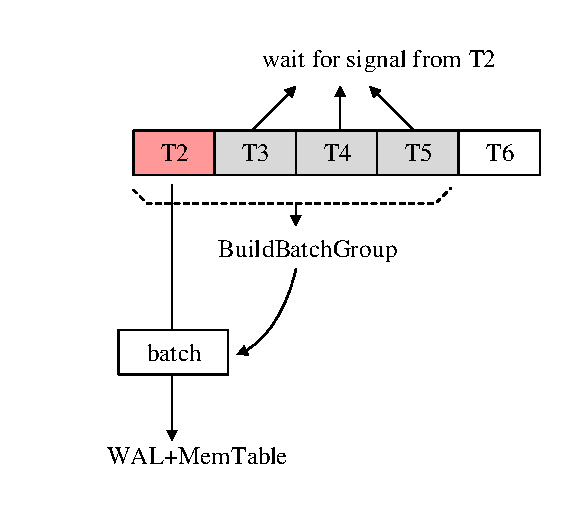
\includegraphics[width=0.5\linewidth]{imgs/leveldb_writebatch.pdf}
	\caption{LevelDB多线程批量写逻辑}
	\label{fig:leveldb_writebatch}
\end{figure}

下面对该流程进行详细分析。初始时\code{writers\_}为空,第一个线程$T_1$进来后不会等待,\code{BuildBatchGroup}返回的batch只包含$T_1$自己。$T_1$在执行\code{mutex\_.Unlock()}语句之后排在后面等待锁的线程$T_2$就可以获得锁并加入到\code{writers\_}。由于$T_2$不在队首所以会执行\code{w.cv.Wait()}在条件变量上等待,此过程会释放\code{mutex\_}上的锁,这样排在后面的$T_3,T_4,...,T_n$就可以按同样的方式获得锁、加入\code{writers\_}等待。当$T_1$完成数据写入后便被移出\code{writers\_}。那么$T_2$是如何被唤醒的?在\code{DBImpl::Write}最后,将batch内的线程唤醒(batch里只有一个$T_1$)后还有一个唤醒操作——将\code{writers\_}队首的线程(也就是$T_2$)唤醒。$T_2$被唤醒后就会把后面若干线程打包进batch。

\subsection{对比}
InfluxDB和LevelDB在处理写请求时都不同程度地采取了group commit。InfluxDB只对WAL进行group commit,而LevelDB对WAL+Memtable都进行group commit,这可能是LevelDB写性能优于InfluxDB的一个原因。

\end{document}
 